\documentclass[spanish, fleqn]{article}
\usepackage[utf8]{inputenc}
\usepackage{graphicx}
\usepackage{amsmath}
\usepackage{bm}
\usepackage{tikz}
\usepackage{adjustbox}
\usepackage[top=3cm,bottom=3cm,left=3.5cm,right=3.5cm,footskip=1.5cm,headheight=1.5cm,headsep=.5cm,textheight=3cm]{geometry}

\begin{document}
\title{Inteligencia Artificial \\ \begin{Large}Estado del Arte: The Progressive Party Problem\end{Large}}
\author{Pablo Ibarra S.}
\date{\today}
\maketitle

\section*{Evaluación}

\begin{tabular}{ll}
Resumen (5\%): & \underline{\hspace{2cm}} \\
Introducción (5\%):  & \underline{\hspace{2cm}} \\
Definición del Problema (10\%):  & \underline{\hspace{2cm}} \\
Estado del Arte (35\%):  & \underline{\hspace{2cm}} \\
Modelo Matemático (20\%): &  \underline{\hspace{2cm}}\\
Conclusiones (20\%): &  \underline{\hspace{2cm}}\\
Bibliografía (5\%): & \underline{\hspace{2cm}}\\
 &  \\
\textbf{Nota Final (100\%)}:   & \underline{\hspace{2cm}}
\end{tabular}

\begin{abstract}
En este informe se presenta un estado del arte del problema conocido como Progressive Party Problem[citar 1]. El problema consiste en programar de la mejor manera una fiesta de yates, donde distintas personas visitaran a varios yates anfitriones. Ademas se definen terminos y conceptos importantes utilizados en la literatura e investigaciones en el área. Se explica y define el problema a tratar, así como también se realizan descripciones y clasificaciones de las distintas variantes que se han desarrollado a través de los años. Se describen las distintas estrategias y algoritmos que se han desarrollado para la resolución del problema principal junto a sus variantes y se presentan también modelos matemticos del problema.
\end{abstract}

\section{Introducción}

Hoy en dia la programacion de horarios es un tema vital para personas y organizaciones, debido a que si se realiza bien, los recursos que se disponen y utilizan, se distribuiran de manera eficiente e inteligente. La programación lineal entera a sido una herramienta clave durante mucho tiempo para resolver este tipo de problemas, aun asi, existen ciertos problemas que PLE(glo) no puede resolver debido a la exploción combinatorial(glo) de estos problemas, un ejemplo de un problema que presenta estas caracteristicas es el problema llamado Progressive Party Problem y sera nuestro foco de estudio en el presente informe.

El problema conocido como Progressive Party Problem fue introducido por Peter Hubbard miembro de la asociación de propietarios SeaWych(link) y del departamento de matematicas de la universidad de Southampton(link), cuando tuvo que organizar una fiesta de yates en la isla Wight, que se encuentra al sur de la costa de Inglaterra. El problema nos situa en el contexto de una fiesta de yates durante la tarde, donde la tripulación de cada yate debe interactuar socialmente con las otras tripulaciones. 

El proposito de este informe es investigar sobre dicho problema, sobre los metodos que existen para solucionarlo, presentar antedeces de lo que se a desarrollado, presentar hacia donde apuntan las nuevas investigaciones y presentar un modelo matematico del problema.

La motivacion de este problema es debido a la importancia que tiene en problemas reales. Inicialmente se planteo como un problema para la organización de fiesta en yates, pero hoy en dia su estudio puede ayudar para organizar de mejor manera ferias de libros, tours y otro tipo de eventos, optimizando los recursos de estos con el fin de maximizar el beneficio, por ejemplo, ganancias.

En este informe se presenta información relevante para poder introducirse al tema de Progressive Party Problem. Primero se comienza definiendo el problema a estudiar y se presentan otras variantes conocidas que existen del problema. Luego le sigue una sección centrada en el Estado del Arte del problema, donde se explican los metodos mas imporatntes que existen de resolucion para este tipo de problemas. Para aportar al estudio del problema este informe presenta, en otra sección, distintos modelos matematicos que pueden ser usados para poder solucionar el problema mediantes tecnicas de optimzacion. Finalmente el informe concluye con unas conclusiones respecto al tema y lo que puede venir en el futuro respecto a este.

\section{Definición del problem}

El problema Progresive Party Problema descrito por Peter Hubbard habla de un total de 39 botes que participan en la fiesta, algunos de estos son seleccionados para ser yates anfitriones, la tripulacion de los yates anfitriones deben mantenerse en su bote ya que tienen que organizar la fiesta en sus barcos, mientras que las otras tripulaciones, que son conocidos como tripulacion huesped, se pasean por los yates anfitriones socializando con el resto de las tripulaciones. La fiesta completa dura 3 horas, por lo que las tripulaciones huespedes deben ir rotando cada 30 minutos para que socializen lo que mas puedan. La tripulacion de cada barco se mantiene junta y cada barco tiene una capacidad maxima. Por otro lado el barco del organizador de la fiesta siempre debe ser anfitrion, independiente de la capacidad del bote, esto es por que en ese barco estaran todos los elementos para enfrentar una eventual emergencia. Debido a que el organizador y dos tripulaciones mas (Estas tripulaciones deberan ser anfitriones y correspoden ser las tripulaciones del bote 1,2 y 3) tienen niños entre sus tripulaciones  se crearon tres botes virtuales con capacidad 0, uno por cada anfitrion, esto se hizo debido a que solo los adultos son anfitriones de los yates designados como anfitriones, por lo tanto el problema final se consideran 42 botes. Finalmente lo que se busca en este problema minimizar la cantidad de barcos anfitriones (debido a que se tienen que abastecer con comida) y asignar las tripulaciones huespedes a cada yate anfitrion durante todos los intervalos de tiempo que dure la fiesta. La Data para el problema dado esta en la siguiente tabla.

\begin{figure}[!h]
  \centering
    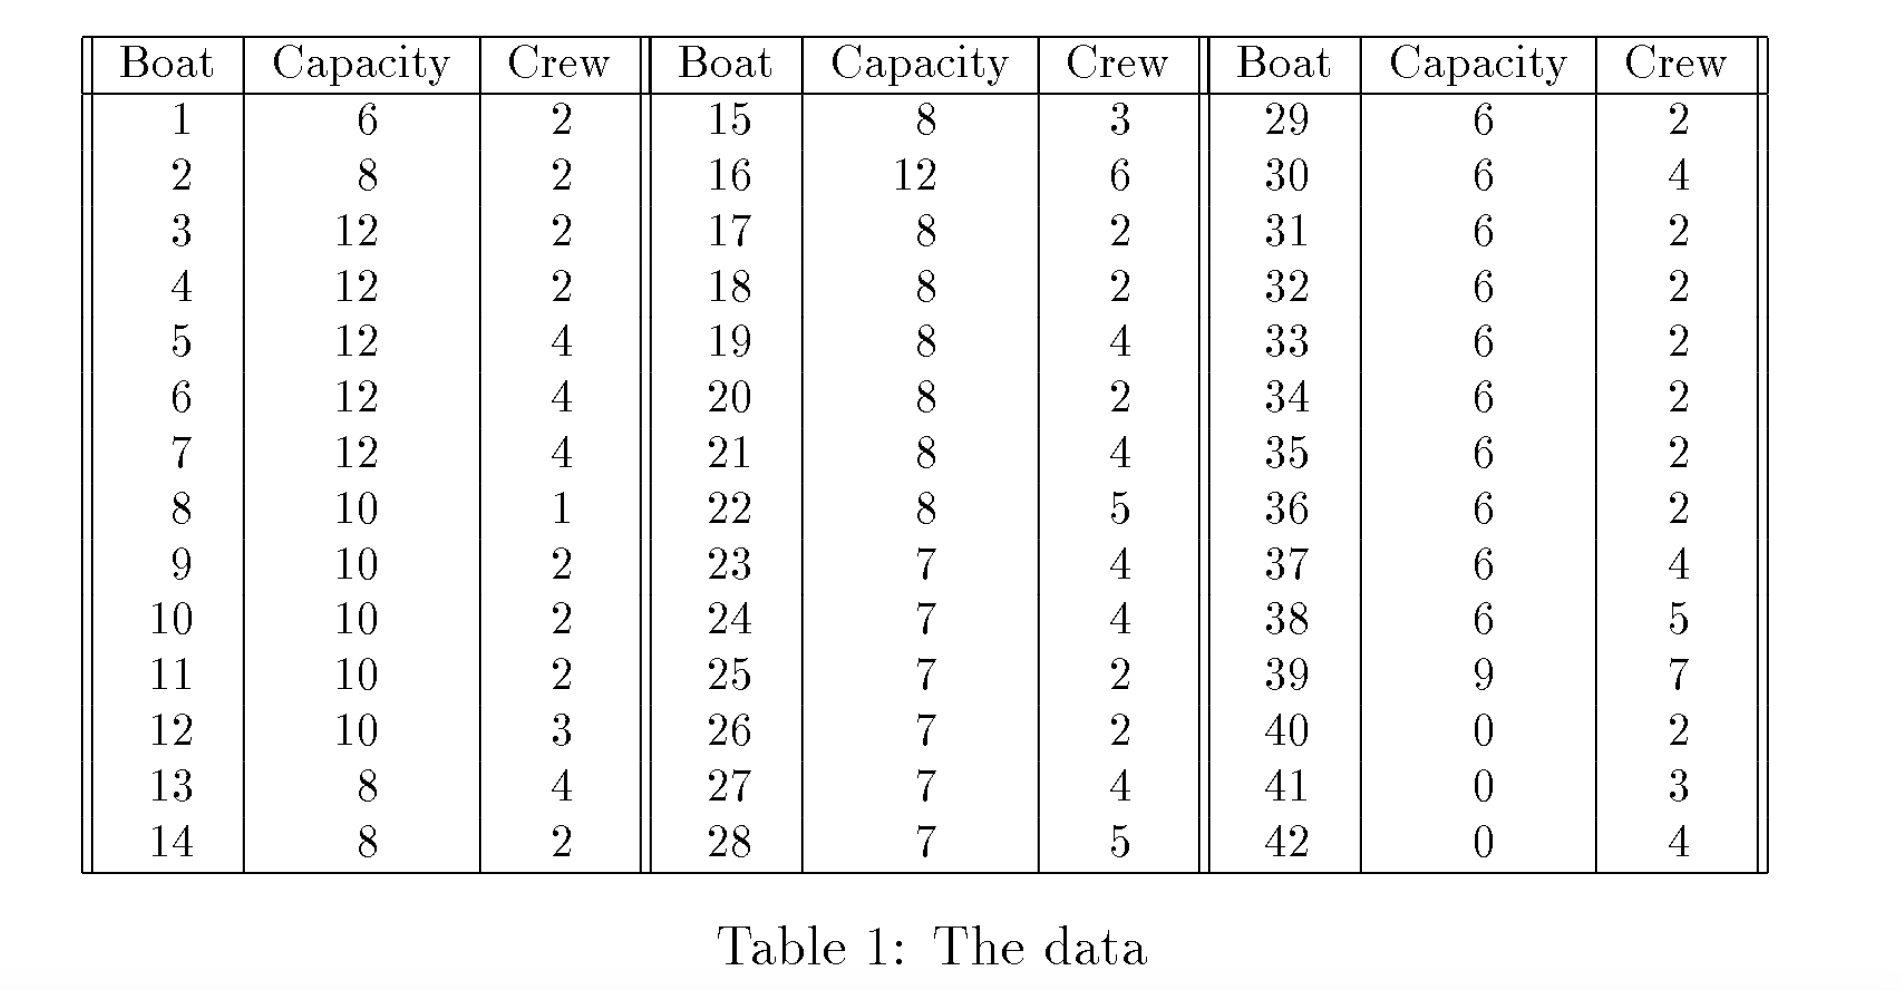
\includegraphics[width=0.7\textwidth]{1}
  \label{fig:DiagramaBarra1}
\end{figure}

\newpage

Por lo tanto identificamos 42 botes (tripulaciones), definimos $\mathit{i},\mathit{j},\mathit{k} \in \{1,..,42\}$ y un conjunto de tiempos $\mathit{t} \in \{1,...,6\}$.

\begin{enumerate}
\item El tamaño de las tripulaciones estara dada por $\mathit{s}_{\mathit{i}}$, y la capacidad del bote - la maxima cantidad de personas que el bote puede recibir incluyendo los dueños del bote es de $\mathit{C}_{\mathit{i}}$.

\item El numero maximo de invitados que puede cada bote invitar es de $\mathit{c}_{\mathit{i}}$ = max (0,$\mathit{C}_{\mathit{i}}$-$\mathit{s}_{\mathit{i}}$).

\item Se introduce la variable binaria $\mathit{x}_{\mathit{i},\mathit{j},\mathit{t}}$. La variable $\mathit{x}_{\mathit{i},\mathit{j},\mathit{t}}$ = 1 si la tripulacion huesped $\mathit{j}$ visita a la tripulacion anfitriona $\mathit{i}$ en el periodo de tiempo $\mathit{t}$. En todo otro caso $\mathit{x}_{\mathit{i},\mathit{j},\mathit{t}}$ = 0.

\item Se utiliza otra variable binaria para decidir cuales botes son anfitriones. La variable $\mathit{h}_{\mathit{i}}$ = 1 si el bote $\mathit{i}$ es anfitrion, en el caso que el bote sea husped $\mathit{h}_{\mathit{i}}$ = 0.

\item Solo hay fiestas en los botes anfitriones, o, si una tripulacion huesped visita a un bote $\mathit{i}$ en algun periodo de tiempo, entonces el bote $\mathit{i}$ es anfitrion.

\item La capacidad maxima de cada bote nunca se puede exceder.

\item No hay tripulaciones hibridas, esto quiere decir que una tripulacion es anfitrion o es huesped.

\item Una tripulacion $\mathit{j}$ visita a otra tripulacion $\mathit{i}$ al menos una vez.

\item Los botes 1,2 y 3 tienen que ser anfitriones. (Barco del organizador y 2 barcos que tenian tripulacion con niños).

\item Los botes 40,41 y 42 deben ser botes huespedes con capacidad 0 (Barco virtual de niños).

\item Las tripulaciones huespedes no pueden encontrarse mas de una vez durante toda la fiesta.

\item Finalmente lo que se busca es minimizar el numero de barcos anfitriones.

\end{enumerate}

El problema 


\bibliographystyle{plain}
\bibliography{Referencias}


\end{document} 